\documentclass{acm_proc_article-sp}
\usepackage{algpseudocode}
\usepackage{verbatim}
\usepackage{microtype}
\usepackage{enumerate}
\usepackage{enumitem}
\usepackage{epsfig}
\usepackage{algorithmicx}
\usepackage{algorithm}
\usepackage{algpseudocode}

\renewcommand{\vec}[1]{\mathbf{#1}}

\begin{document}

\title{A Comparative Study of the Echo State Networks}

\numberofauthors{2}
\author{
\alignauthor
Rob Argue\\
       \affaddr{University of Maryland}\\
       \affaddr{Department of Computer Science}\\
       \email{rargue@cs.umd.edu}
% 2nd. author
\alignauthor
Joshua Bradley\\
       \affaddr{University of Maryland}\\
       \affaddr{Department of Computer Science}\\
       \email{jgbrad1@cs.umd.edu}
}

\maketitle
\begin{abstract}
In this study, we compare the performance and behavior of an echo state network (ESN) to several recurrent neural network architectures, including the Elman network, Jordan network, and feedforward network, when applied to the task of nonlinear time series forecasting. We will describe several benchmark tests used and provide a discussion of the results.
\end{abstract}

\section{Introduction}
Recurrent Neural Networks (RNNs) have been shown to be effective function approximators in time series prediction. One of the disadvantages to applying RNNs to various prediction tasks though is the increased computational cost required to train such networks to a sufficient error threshold. This is due to the network architecture design, in which every node in the hidden layer(s) is conventionally considered to be fully inter-layer connected (i.e. Elman networks, Jordan networks). Recently, Echo State Networks (ESNs) have been shown to be quite effective at similar tasks, yet not require such great computation cost. In this study, we compare the performance and behavior of ESNs to two other popular recurrent neural network architectures (Elman, Jordan). Also, we give a quick performance comparison of ESNs and feeforward networks. Jordan network, and feedforward network, when applied to the task of nonlinear time series forecasting. We will describe several benchmark tests used and provide a discussion of the results.

\section{Data}
Selection of the dataset is very important in our study. To ensure a fair comparison of the echo state network and other RNN architectures when applied to time series forecasting, datasets exhibiting specific traits must be chosen. The traits we have chosen to base data selection on include
\begin{itemize}
\item Degree of periodicity - For example, a dataset of household electricity consumption would be expected to exhibit reasonably normal daily periodic patterns while a dataset of certain stock prices may be expected to exhibit annual periodic behavior.
\item Amount of bias/variance within the data - For example, stock pricing depends on a large number of factors in the market to be considered, thus it is expected to exhibit a greater amount of variance and bias vs. a dataset of daily household electricity consumption.
\end{itemize}
Three data sets were used for each of the experiments. The time delay differential Mackey-Glass equation,
\begin{equation*}
\frac{dx}{dt} = \beta \frac{x_\gamma}{1+x_{\gamma}^n} - \gamma x \text{  for  } \gamma, \beta, n \ge 0
\end{equation*}
was used to generate the first set of data, using a time delay of 17, which comprised a chaotic time series with no additional features. Stock market data [1] was used for a time series with several features. For the purpose of these experiments we took the finance sector portfolio to be the target data, and the other sectors to be features. A household power consumption data set [2] was used as an example of a time series with some missing data, which we decided to treat as noise. For each dataset, all data was normalized to the range $[-1,1]$. The expectation was that the ESN would perform best on the Mackey-Glass data and worst on the power consumption data.

\section{Methodology}

For the ESN, we decided to use the following structure.
\begin{figure}[here]
\begin{center}
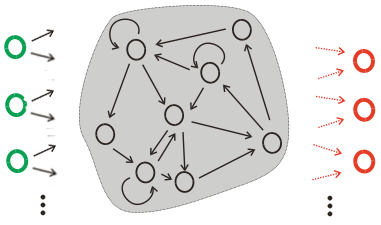
\includegraphics[scale=0.35]{ESNStructure.png}
\caption{ESN architecture}
\end{center}
\label{fig:esn_structure}
\end{figure}
There exist many variants of the ESN. For the best comparison of the ESN and Elman network, we felt it would be most appropriate to employ a design where recurrent connections exist only in the reservoir. The ESN was constructed and trained in the following manner.
\begin{enumerate}
\item Generate an untrained dynamical reservoir network by computing random values for the weight matrices $\vec{W}^{in}$, $\vec{W}$, $\vec{W}^{back}$.
\item Ensure the reservoir has the echo state property and displays mutually different dynamics upon excitement. This was done by populating $\vec{W}$ with random values in the range $[-1, 1]$ and setting
\begin{eqnarray*}
W = \frac{\alpha}{|\lambda_{max}|} W
\end{eqnarray*}
where $\lambda$ is the eigenvalue of $W$ and $\alpha \in (0,1)$ a user-defined spectral radius.
\item Arbitrarily initialize the network state $\vec{x}(0)$.
\item For time $t = 0 \ldots T$, run each input pattern $\vec{u}(t)$ and target output $\vec{d}(t)$ through the ESN, updating the network by
\begin{eqnarray*}
\vec{x}(t+1) = \vec{f}(\vec{W}^{in} \vec{u}(t+1) + \vec{W} \vec{x}(t))
\end{eqnarray*}
where f is any sigmoidal activation function. For our experiments, we define f = $\tanh$. If trained output-to-reservoir connections are used, then updating the network would require
\begin{eqnarray*}
\vec{x}(t+1) = \vec{f}(\vec{W}^{in} \vec{u}(t+1) + \vec{W} \vec{x}(t) + \vec{W}^{back} \vec{d}(t))
\end{eqnarray*}
\item Once a particular amount of washout time has passed, begin collecting network states in a matrix $\vec{C}$ row-by-row where each row is a concatenation of the vectors $(\vec{u}(t), \vec{x}(t))$. Also store the target output into each row of a matrix T as $\vec{f}^{-1}(\vec{d}(t))$. In our case, this was $\tanh^{-1}(\vec{d}(t))$.
\item To calculate $\vec{W}^{out}$, the final step is to compute the pseudoinverse of the matrices $\vec{C}$ and $\vec{T}$.
\begin{eqnarray*}
(\vec{W}^{out})^\top = \vec{C}^{-1} \vec{T}
\end{eqnarray*}
\end{enumerate}

After training, to test for time series predictions, all one must do is run the following update equations
\begin{eqnarray*}
\vec{x}(t+1) &=& \vec{f}(\vec{W}^{in} \vec{u}(t+1) + \vec{W} \vec{x}(t)) \\
\vec{y}(t+1) &=& \vec{f}(\vec{W}^{out} (\vec{u}(t+1), \vec{x}(t+1), \vec{y}(t))) \\
\end{eqnarray*}


\section{Experiments}
In the analysis of our ESN three experiments were run. The initial experiment was parameter optimization of the ESN, and sought to explore the effects of network architecture and learning rule parameters on the performance of the model. Performance was measured as mean square error of ESN output and actual data for a test set of data which immediately suceeded the training data. Lastly a comparison of run time of the networks was conucted using the power consumption data set.

Parameter optimizaation was run with the parameters $leakRate$, $reservoirSize$, $spectralRadius$, and $forgetSize$. For each data set each parameter was varied independantly of the others, and were held at default values of
$$leakRate = 0.5$$
$$reservoirSize = 100$$
$$spectralRadius = 0.5$$
$$forgetSize = 100$$

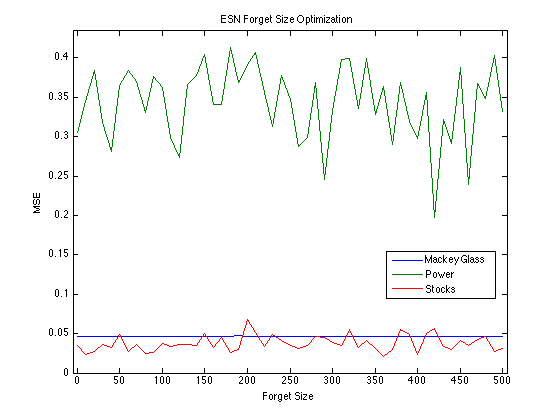
\includegraphics[scale=0.7]{ForgetSizeOptimization.png}
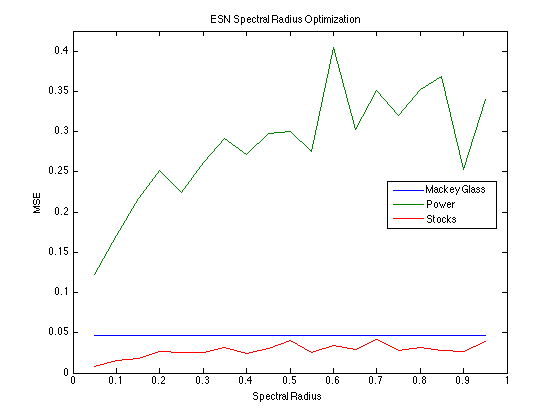
\includegraphics[scale=0.7]{SpectralRadiusOptimization.png}
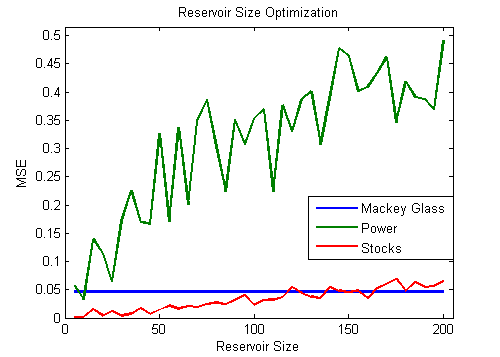
\includegraphics[scale=0.7]{ReservoirSizeOptimization.png}
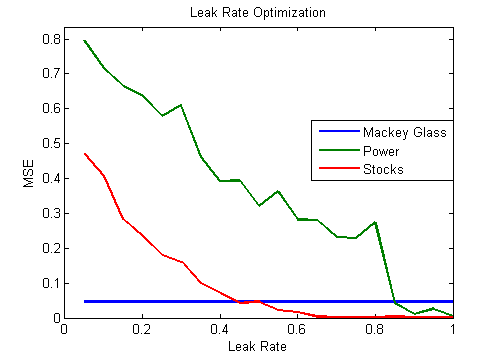
\includegraphics[scale=0.7]{LeakRateOptimization.png}

For all of the parameter, the Mackey-Glass performance stayed constant, which is consistant with what we saw for other networks. $forgetSize$ appearned to have little to no effect on the performance of the ESN, while the expectation was that there would be higher towards 0, which would quickly drop to a stable value. The ESN tended to perform better with smaller $spectralRadius$.  $reservoirSize$ similarly had a positive correlation with error, which is the opposite of expectation.  The decay of error with a higher $leakRate$ matched what we expected to happen.  Possible explanations for these results not matching our hypothesised results are (JOSH PUT SOMETHING HERE I DON'T KNOW).

In the second experiment we compared our ESN to other, commercially available neural networks. In particular we compared it to a feedforward network as a control, and to Elman and Jordan networks as examples of other recurrent nets. Matlab's Neural Network Toolbok was used for these networks. All three of the comparison networks were trained using RProp, and a best of three runs approach was taken in attempt to minimize the effect of outliers. We varied the size of the hidden layer (the reservoir in the case of our ESN) for some variety in architecture. The ESN used parameters optimized to each data set, while the other networks used default Matlab parameters in the interest of time.

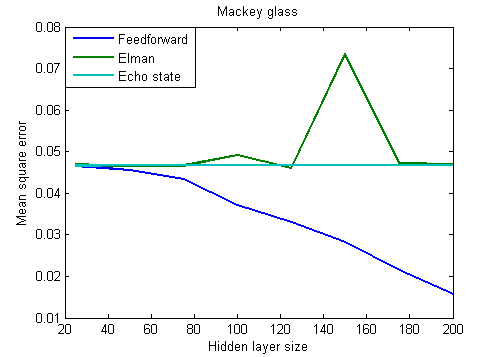
\includegraphics[scale=0.7]{mackey_plot.png}
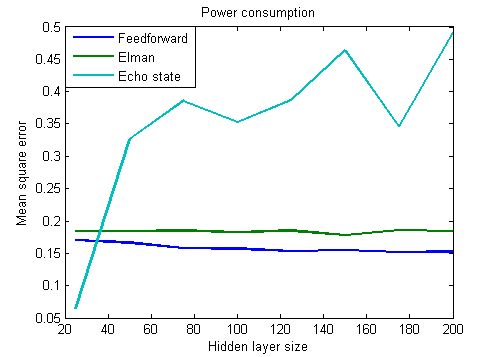
\includegraphics[scale=0.7]{power_plot.png}
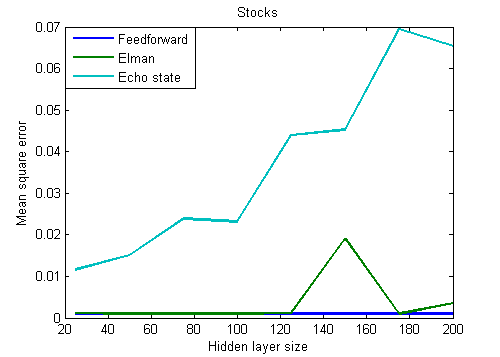
\includegraphics[scale=0.7]{stocks_plot.png}

The ESN performed best on the Mackey glass dataset, proving to be approximately equal to the Elman net, though with significantly higer consistancy, which matches with our expectations. For the power consumption dataset, the ESN performed somewhat poorer than the feedforward and Elman nets, with approximately double the error. On the stocks dataset the ESN performed significantly worse than the feedforward and Elman nets. This seems to indicate a general trend that the ESN performs more comparably on datasets which have fewer features, and instead tend to be more pure functions of time. Contrary to our initial hypothesis, did not seem to perform significantly worse compared to the other networks on the data set with missing data (the power consumption data set). 

The run time experiment was conducted under the same circumstances as the second experiment, however was only run on the power data set, and only one run was made for each data point.

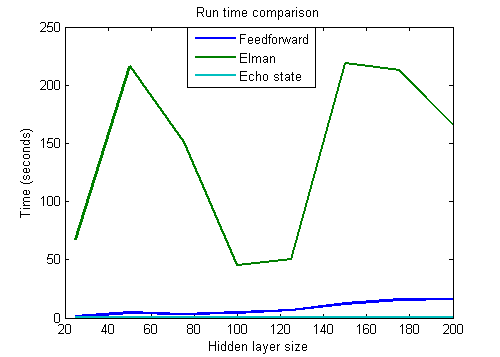
\includegraphics[scale=0.7]{time_plot.png}

The ESN took significantly less time to train, especially with a larger network size, running orders of magnitude faster than the Elman net, even at a small network size.

\section{Future Work}
Our ESN also has the ability to have output to reservoir connections, which we felt would be good to include for a comparison to Jordan nets. We were unable to finish debugging the Jordan nets in time to be able to conduct this comparison, so it is being left as future work. Additionally, parameter optimization for the Matlab nets should be performed, and other learning meathods for them would be interesting to investigate. Our ESN could also be adapted to work on multiple time series, and comparisons could be done with those.

\section{Conclusions}
Our ESN performed reasonably well as compared to other simple recurrent nets. In general the ENS net tended to have somewhat worse performance, especially on featured data, but took a significantly shorter time to train, and was less prone to getting stuck in bad local minima, especially as compared to the Elman net. (WHAT ELSE DO YOU WANT TO SAY HERE?)

\bibliographystyle{abbrv}
\bibliography{sigproc}

\balancecolumns
\end{document}
